\documentclass[sigconf]{acmart}

\usepackage{booktabs} % For formal tables
\usepackage{epstopdf} % For eps
\usepackage{url}
\usepackage[T1]{fontenc}
\usepackage{float}

% Copyright
%\setcopyright{none}
%\setcopyright{acmcopyright}
%\setcopyright{acmlicensed}
\setcopyright{rightsretained}
%\setcopyright{usgov}
%\setcopyright{usgovmixed}
%\setcopyright{cagov}
%\setcopyright{cagovmixed}


% DOI
\acmDOI{XX.XXX/XXX_X}

% ISBN
\acmISBN{XXX-XXXX-XX-XXX/XX/XX}

%Conference
\acmConference[WebMedia'2017]{Brazilian Symposium on Multimedia and the Web}{October 2017}{Gramado, RS Brazil} 
\acmYear{2017}
\copyrightyear{2017}

\acmPrice{15.00}


\begin{document}
\title{CrowdSub: a crowdsourcing system for video subtitling}
%\titlenote{Produces the permission block, and
 % copyright information}
%\subtitle{a Crowdsourcing Approach}
%\subtitlenote{The full version of the author's guide is available as
%  \texttt{acmart.pdf} document}


\author{Removed for double-blind review}
%\authornote{Dr.~Trovato insisted his name be first.}
%\orcid{1234-5678-9012}
\affiliation{%
  \institution{Removed for double-blind review}
%  \streetaddress{Removed for double-blind review}
 % \city{Removed for double-blind review} 
  %\state{Removed for double-blind review} 
  %\postcode{Removed for double-blind review}
}
\email{Removed-for-double-blind-review}

\author{Removed for double-blind review}
%\authornote{Dr.~Trovato insisted his name be first.}
%\orcid{1234-5678-9012}
\affiliation{%
  \institution{Removed for double-blind review}
 % \streetaddress{Removed for double-blind review}
  %\city{Removed for double-blind review} 
  %\state{Removed for double-blind review} 
  %\postcode{Removed for double-blind review}
}
\email{Removed-for-double-blind-review}

\author{Removed for double-blind review}
%\authornote{Dr.~Trovato insisted his name be first.}
%\orcid{1234-5678-9012}
\affiliation{%
  \institution{Removed for double-blind review}
  %\streetaddress{Removed for double-blind review}
  %\city{Removed for double-blind review} 
 % \state{Removed for double-blind review} 
 % \postcode{Removed for double-blind review}
}
\email{Removed-for-double-blind-review}


% The default list of authors is too long for headers}
\renewcommand{\shortauthors}{Removed for double-blind review}


\begin{abstract}
	TO DO

\end{abstract}

%
% The code below should be generated by the tool at
% http://dl.acm.org/ccs.cfm
% Please copy and paste the code instead of the example below. 
%
\begin{CCSXML}
<ccs2012>
<concept>
<concept_id>10002951.10003260.10003282.10003296</concept_id>
<concept_desc>Information systems~Crowdsourcing</concept_desc>
<concept_significance>500</concept_significance>
</concept>
<concept>
<concept_id>10003120.10003130.10003131.10003570</concept_id>
<concept_desc>Human-centered computing~Computer supported cooperative work</concept_desc>
<concept_significance>500</concept_significance>
</concept>
<concept>
<concept_id>10010405.10010497.10010510.10010513</concept_id>
<concept_desc>Applied computing~Annotation</concept_desc>
<concept_significance>500</concept_significance>
</concept>
<concept>
<concept_id>10002951.10003227.10003251</concept_id>
<concept_desc>Information systems~Multimedia information systems</concept_desc>
<concept_significance>500</concept_significance>
</concept>
<concept>
<concept_id>10003120.10003121.10003124.10010868</concept_id>
<concept_desc>Human-centered computing~Web-based interaction</concept_desc>
<concept_significance>500</concept_significance>
</concept>
<concept>
<concept_id>10003120.10011738</concept_id>
<concept_desc>Human-centered computing~Accessibility</concept_desc>
<concept_significance>300</concept_significance>
</concept>
</ccs2012>
\end{CCSXML}

\ccsdesc[500]{Information systems~Multimedia information systems}
\ccsdesc[500]{Human-centered computing~Web-based interaction}
\ccsdesc[500]{Information systems~Crowdsourcing}
\ccsdesc[500]{Human-centered computing~Computer supported cooperative work}
\ccsdesc[500]{Applied computing~Annotation}
\ccsdesc[300]{Human-centered computing~Accessibility}



\keywords{Crowdsourcing, Video Annotation, Human Computation, Microtasks, Multimedia Systems, Video Enrichment, Caption, Subtitle, Accessibility}


\maketitle

\section{Introduction}
	TO DO


REFS:

Crowdsourcing video enrichment \cite{162960}

Wisdom of Crowds \cite{Howe2006,GALTON1907}

Human Computation \cite{vonAhn:2011:THC}

Microtasks \cite{Difallah:2015:DMC:2736277.2741685,Chen:2017:RIM:3025453.3025969}

\section{Crowdsourcing Workflow}
	
\begin{figure}[h]
	\centerline{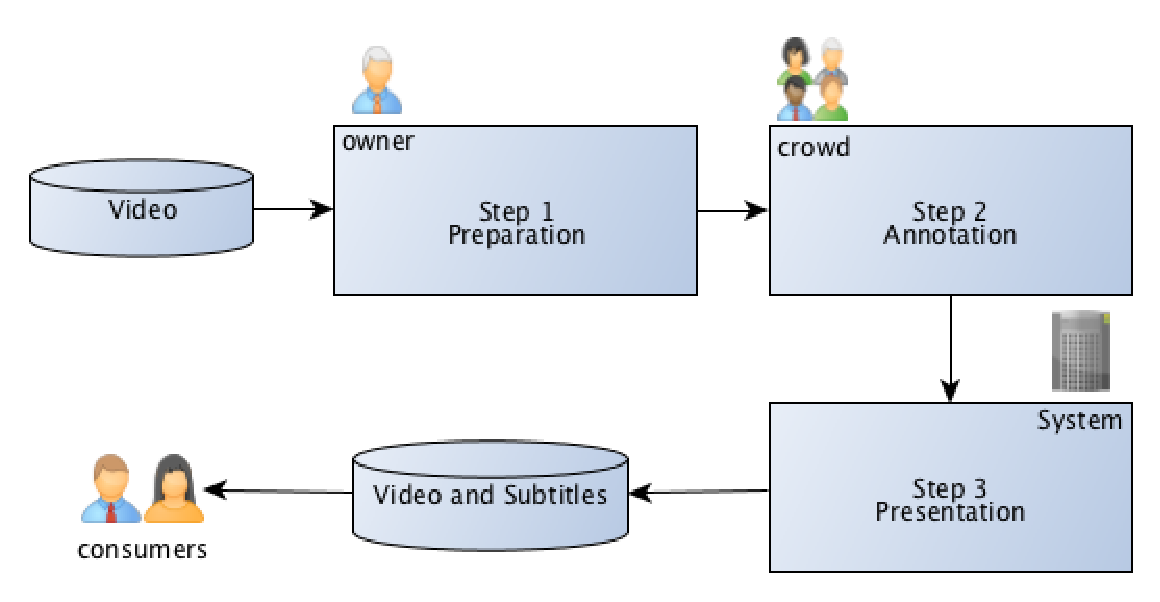
\includegraphics[scale=0.4] {figure/workflow-01}}
	\caption{Process workflow}
	\label{process}
\end{figure}


\section{System Design}
	TO DO

\section{Experiment}
	TO DO

\section{Conclusion}
	TO DO

\begin{acks}
Removed for double-blind review.
\end{acks}



\bibliographystyle{ACM-Reference-Format}
\bibliography{refs} 

\end{document}
